\startchapter{Modelling of Signal and Background Processes}
\label{chapter:mc}

To search for evidence of new physics in the ATLAS data, it is necessary to develop an accurate model of the expected yield of both SM events (a.k.a. ``background") and hypothesized BSM events (a.k.a. ``signal") in the data, as well as their kinematic distributions. The yields and kinematic distributions of events in the data are then compared with those in the signal and background model to check for any ``above-background" significant excesses in the data that could point to the presence of BSM physics. If no significant excesses are observed, the search can exclude the signal model for the range of signal model parameters for which the model predicts a significant above-background excess in the data.

Like many collider experiments, the ATLAS collaboration uses a method called ``Monte Carlo" (MC) to model the expected yield and kinematic distributions of SM and hypothesized BSM events in the data collected by the detector. The MC method is a computational algorithm which uses repeated sampling of random variables, where each set of randomly sampled variables represents a randomly generated ``event". For each event, the random variables associated with the event are passed into the model to produce a resulting set of output variables. For physical models, one is particularly interested in the set of ``observable" output variables, meaning those which can be measured experimentally in the modelled system. The method is useful for complex models with many free parameters, and for which it would be unfeasible to develop analytical formulations of the distributions of observables predicted by the model. 

Given a set of MC simulated events, the associated set of values for each observable generated by passing the events through the model represents a random sampling of the underlying probability density distribution for that observable according to the model. The events can be binned into histograms in one or more observables. Assuming that, for each event, the sampling of random variables is performed ``independently" - i.e. in a manner such that the sampling of random variables for each event is unaffected by that of any other event - the number $N_i$ of events in each bin $i$ will vary randomly according to Poisson statistics with, on average, a standard deviation of $\sigma_{N_i}=\sqrt{N_i}$. Consequently, as the number of MC simulated events is increased by a factor of $\alpha$, the relative size $\frac{\sigma_{N_i}}{N_i}$ of fluctuations in each bin will, on average, decrease according to $\frac{1}{\sqrt{\alpha}}$. As a result, as one increases the number of MC simulated events, the shapes of histograms binned in the model's observables for the simulated events will become an increasingly precise approximation of the underlying probability distributions for these observables according to the model. 

Signal and SM background models used to perform searches for BSM physics with the ATLAS detector are produced using sophisticated MC simulations of both the passage of the final-state particles through the ATLAS detector and of the physical production mechanisms for the particle collision, production and decay processes involved. For a given process, for example the dominant \wjets background in this DM search shown in Figure \ref{fig:Wjets_Feynman}, ``truth-level" information for each MC event is first obtained from a random proton-proton collision by simulating the physical production mechanism for the process. The set of simulated final state particles, along with their kinematic information, are collectively known as the ``truth-level" event. Truth-level events can subsequently be passed through a highly detailed  simulation of the ATLAS detector \cite{atlas_sim} produced using the Geant4 toolkit \cite{Geant4}, which models how these events would actually be measured by the detector at ``reconstruction-level". ATLAS requires very large MC data sets (millions of simulated events per process) to adequately model the predicted probability distributions for kinematic observables over their full range of interest for the measurements of SM and BSM searches that use the ATLAS data.

ATLAS uses various MC simulation packages (also known as ``generators") to perform truth-level MC simulation of different physics processes. For many processes, particularly SM background processes, independent MC simulations have been performed using several different packages, and the yields and distributions of events predicted by the different packages can be compared to evaluate a systematic uncertainty associated with the choice of generator used to simulated the process. The specific generators used to model the physics processes considered in this search will be discussed in Sections \ref{sec:DH_model_sim} and \ref{sec:SM_bkg_sim}.

\section{Weighting and Normalization of MC Simulated Processes}

To produce an accurate prediction of the yield and distributions of events in the actual ATLAS data set, it is necessary to apply individual event-level weights and overall normalization factors to the MC simulated events, as described in the following sections.

\subsection{Weighting of MC Simulated Events}
\label{sec:evt_wts}

At various stages of the MC simulation procedure, multiplicative weight factors - or simply ``weights" - are calculated and saved for each event. These weights modify the amount by which a given event contributes to the amplitude of the bin that it gets assigned to relative to other events when the MC simulated events are binned into histograms. For a given process, the overall factor which is applied to weight each event relative to other events generated for the same process is given by the product of ``event-level weights", which are designed to apply corrections arising from various aspects of the event generation and reconstruction. 

For each event $i$, the total event-level weight is given by the following product:

\begin{multline}
\label{eq:evt_wt}
\text{event-level weight }i = \text{(generator weight)}_i \times \text{(pileup reweighting weight)}_i \times \\ \times \prod_j \text{(reconstruction weight j)}
\end{multline}

The ``generator weight" is a weight applied by some generators during the generation of truth-level events for various purposes. These purposes may include correcting for the generation of duplicate events at different stages of the calculation, correcting leading-order calculations to achieve the expected distributions that a more precise ``next-to-leading-order" calculation would be expected to produce. 

The ``pileup reweighting weight" is designed to account for the effects of ``pileup" \cite{pileup}, where pileup constitutes the soft QCD collision events that take place in the same (or closely-surrounding) bunch crossings as the ``hard interaction" that actually triggered the event readout. The nominal procedure of simulating the ``hard interactions" which would produce the process being modelled does not account for the presence of these pileup interactions that would be measured by the detector as part of the readout for the hard interaction of interest. Instead, a dedicated weighting factor, the so-called pileup reweighting weigh, is applied to each simulated event such that the overall normalization and shapes of observables in the MC data set properly reflects the actual pileup conditions present over the full Run 2 data-taking period.

The ``reconstruction weights" collectively refer to weights assigned to apply corrections associated with the reconstruction of objects such as electrons, muons and jets that would be produced when simulating the passage of the event through the ATLAS detector.

\subsection{Scaling Distributions for Comparison with Data}

In addition to the event-level weights described in Section \ref{sec:evt_wts} above, scaling factors are applied to each signal and background process such that the amplitude - i.e. predicted number of events per bin - of the MC distributions for each process properly predict the actual yield of events expected in the ATLAS data. 

\subsubsection{Sum of Weights Normalization}

As a first step, the MC weights of all events in each process are divided by the sum over all event weights for the process, such that these normalized event weights sum to 1: 

\begin{multline}
\label{eq:evt_wt_norm}
\text{event-level weight (normalized) }i =\frac{\text{event-level weight }i }{\sum_j \text{event-level weight }j }
\end{multline}

\noindent where the index j runs over all events in the process.

\subsubsection{Scaling to Expected Data Yield}

As discussed in Section \ref{sec:decay_processes}, the total predicted yield \(N\) of events for a given process of particle production and decay initiated by a proton-proton collision in the LHC is given by:

\begin{equation}
\label{eq:predicted_yield}
N = \sigma\int_{t_1}^{t_2}\mathcal{L}(t)dt = \sigma\mathcal{L}_\text{int}
\end{equation}

\noindent where \(\int_{t_1}^{t_2}\mathcal{L}(t)dt\) is the integrated beam luminosity over the full data-taking period from \(t_1\) to \(t_2\) and \(\sigma\) is the cross section for the process, which quantifies the probability that the process will occur, relative to other processes that could also be initiated by the proton-proton collisions. 

Therefore, the final step in weighting the MC events for comparison with data is to scale all the normalized MC weights in Eq. \ref{eq:evt_wt_norm} by the product of the cross section \(\sigma\) for the given process and the integrated ATLAS luminosity \(\mathcal{L}_\text{int}\) such that they sum to the total predicted yield \(N\) of events for the process:

\begin{equation}
\label{eq:evt_wt_norm_scale}
\text{event-level weight (normalized, scaled) }i = \text{event-level weight (normalized) }i \times \sigma \times \mathcal{L}_\text{int}
\end{equation}

\noindent Summing all event weights in Eq. \ref{eq:evt_wt_norm_scale}, and combining with \ref{eq:evt_wt_norm} and \ref{eq:predicted_yield} produces the total predicted yield for the given process:

\begin{multline}
\label{eq:evt_wt_sum}
\sum_i\text{event-level weight (normalized, scaled) }i = \frac{\sum_i \text{event-level weight }i}{\sum_j \text{event-level weight }j}\times \sigma \times \mathcal{L}_\text{int} \\
 = \sigma\mathcal{L}_\text{int} = N
\end{multline}

\section{Comparing Data and MC to Search for New Physics}

With the MC simulated data properly weighted and normalized as described in Section \ref{sec:evt_wts} above, event selections are applied to both data and MC based on their final-state observables, such as the identity, momenta and directions of final-state particles measured by the detector. The selections, which are discussed in more detail in Section \ref{sec:evt_selections}, are designed to define one or more regions of the data, known as ``signal regions" within which the signal MC predicts a relatively large yield of a hypothesized new physics process compared with the MC prediction of SM background processes. Within each signal region, the data and MC may be additionally binned in one or more final-state observables, and the resulting distributions of ATLAS data are compared with those of the total MC simulated SM background yields to check for any significant yield excesses or shape differences in ATLAS data which could be indicative of new physics.

\section{Simulation of the DH Signal Model}
\label{sec:DH_model_sim}

Presentation of signal grid and simulation details (eg. leading Feynman diagrams, use of FullSim, inclusion of additional final-state jet, etc.).

The DH signal model presented in Chapter \ref{chapter:dh_model} is simulated by using a program called MadGraph 5 \cite{MG5}\footnote{\MGNLO[2.7.2](ATLAS, LCG)~\cite{Alwall:2014hca} is the particular version of MadGraph 5 used to generate the MC signal data used in this search.}, which generates proton-proton collision events and calculates the matrix element at leading order to produce events associated with the Lagrangian for a given process. The Lagrangian for the dark Higgs signal model is encoded in MadGraph, with the coupling constants \(g_q\), \(g_\chi\), the mixing angle \(\theta\), and the DM mass \mchi fixed to the values specified in Chapter \ref{chapter:dh_model}. The DH and \Zprime masses \ms and \mZp are left as floating parameters in the search. Therefore, MC data is generated over a grid of \ms and \mZp over which the search is expected to be reasonably sensitive to the model. Figure \ref{fig:signalgrid} shows the \ms and \mZp masses for which MC data sets were generated for the DH signal process. 

\begin{figure}[h]
	\centering
	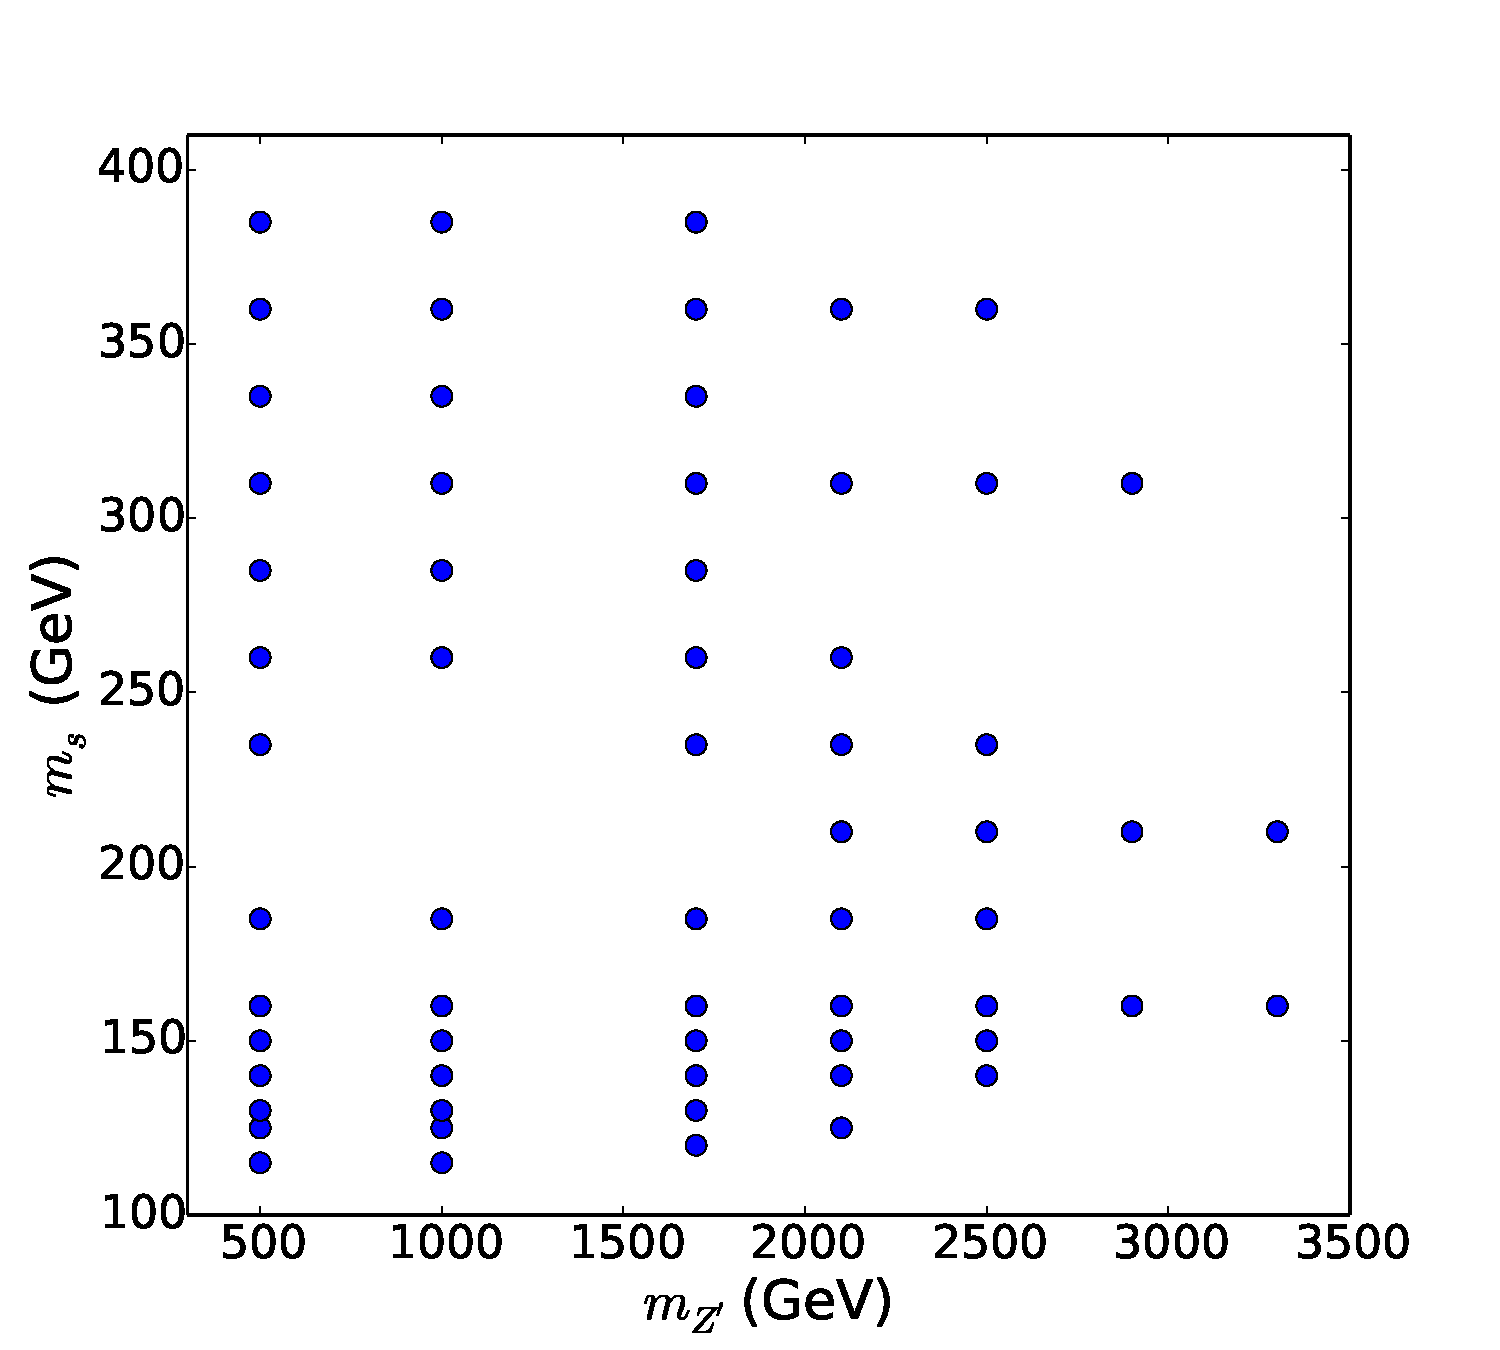
\includegraphics[width=0.8\textwidth]{Figures/4/Grid.pdf}
	\caption{Grid of produced signal samples with different choices of \mZp, \ms and the other parameters fixed to \(g_{q}=0.25\), \(g_{\chi} = 1.0\), \mchi = 200 GeV, \(\theta = 0.01\). Signal points generated in the on-shell \(s\rightarrow WW\) decay regime of \(\ms \geq 160\) GeV are shown in blue, and points generated with \ms below this on-shell \(WW\) production regime are shown in red.}
	\label{fig:signalgrid}
\end{figure}

As discussed in Chapter \ref{chapter:dh_model}, the signal model considered in this search produces two final-state partons from the \(s \rightarrow WW(qq\ell\nu\) decay. MadGraph also includes production mechanisms in the matrix element calculation for which up to one additional parton is radiated in the final state. These final-state partons initiate cascades of radiation produced by QCD processes \cite{parton_shower}, which are modelled using the Pythia8\footnote{The \PYTHIA[8.230]\cite{Sjostrand:2014zea} is the particular version of Pythia8 used to generate the MC signal data used in this search.} program

\section{Simulation of SM Background Processes}
\label{sec:SM_bkg_sim}

The selection criteria applied to final-state observables in the ATLAS and MC data are designed to define signal regions which contain events that exhibit the final-state signature of the the DH signal model, namely of a \(WW\) pair which decays semileptonically and recoils against missing transverse momentum. However, some SM processes can result in final state observables which are similar enough to that of the signal model as to produce an appreciable yield of events in the signal regions. In addition to targeting the signal model, the selections are also optimized to minimize the predicted yield of SM background processes in the signal regions. This section presents the background processes which still have a non-negligible yield in the signal regions even with the optimized signal region selections.

Dominant backgrounds to the search are \wjets, Diboson and \ttbar processes described in Sections 
The \wjets and \ttbar processes are estimated by MC simulation in combination with the use of data-driven control region to constrain the background normalization in the combined fit.
Other backgrounds are estimated purely by simulation.

Figure \ref{fig:background_yield_breakdown} shows the yield breakdowns in the signal regions of all SM background processes considered in the analysis.

\begin{figure}[h]
  \centering
     \begin{subfigure}{0.49\textwidth}
     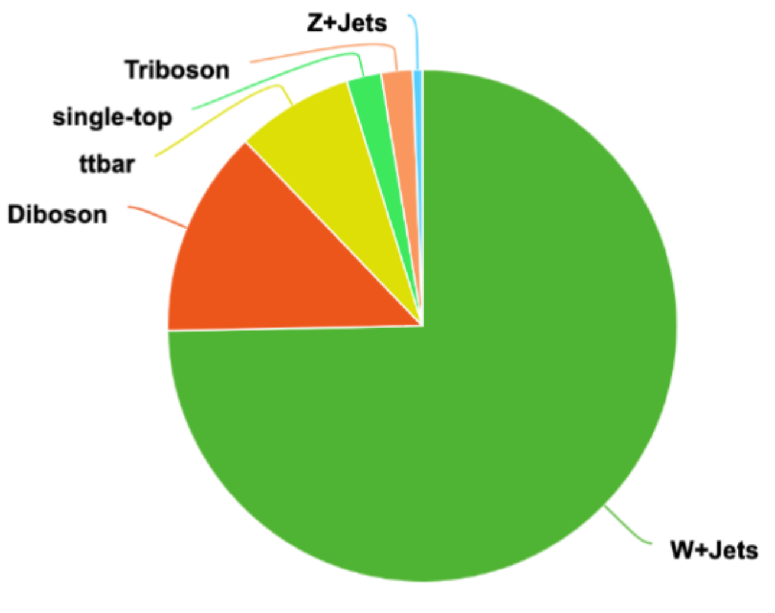
\includegraphics[width = 0.98\textwidth]{figures/4/background_yield_breakdown_merged_SR.pdf}
    \caption{\merged SR}
    \label{fig:background_yield_breakdown_merged_SR}
     \end{subfigure}
    \begin{subfigure}{0.49\textwidth}
     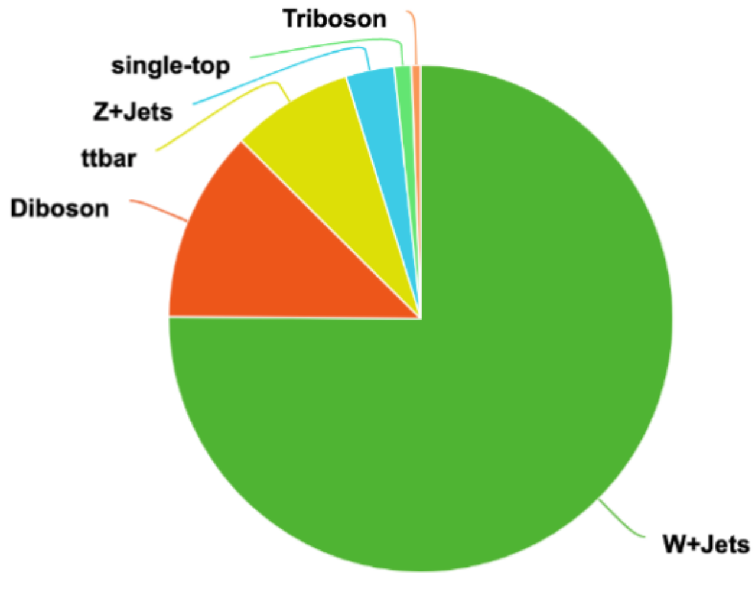
\includegraphics[width = 0.98\textwidth]{figures/4/background_yield_breakdown_resolved_SR.pdf}
     \caption{\resolved SR}
     \label{fig:background_yield_breakdown_resolved_SR}
     \end{subfigure}
     \caption{Relative contribution of all SM background processes considered in the signal regions}
     \label{fig:background_yield_breakdown}
  \end{figure}


\subsection{Dominant Background Processes}

\subsubsection{\wjets}
\label{sec:wjets_description}

The dominant SM background in the signal regions comes from the \wjets process, wherein a leptonically decaying \(W\) is produced from the initial parton-parton collision, along with hadronic activity which fakes the hadronically decaying \(W\) in the signal model. A leading Feynman diagram for the \wjets background is shown in Figure \ref{fig:Wjets_Feynman}.

\begin{figure}[h]
  \centering
     \begin{subfigure}{0.49\textwidth}
     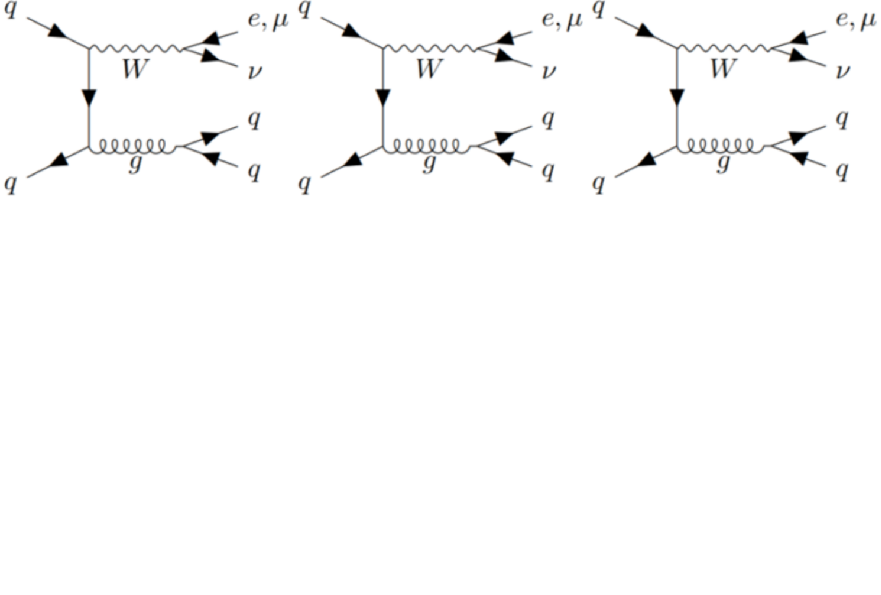
\includegraphics[width = 0.75\textwidth]{Figures/4/Fey_Wjets.pdf}
    \caption{\wjets}
    \label{fig:Wjets_Feynman}
     \end{subfigure}
    \begin{subfigure}{0.49\textwidth}
     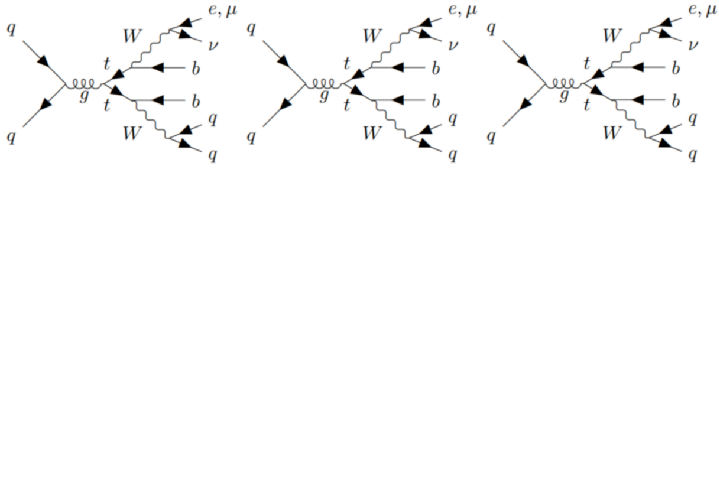
\includegraphics[width = 0.75\textwidth]{Figures/4/Fey_ttbar.pdf}
     \caption{\ttbar}
     \label{fig:ttbar_Feynman}
     \end{subfigure}
     \caption{Feynman diagrams for \wjets and \ttbar SM background processes}
     \label{fig:Feynman_bkgs}
  \end{figure}
  
The \SHERPA[2.2]~\cite{Gleisberg:2008ta} MC generator is used to model both the hard \wjets process, as well as the parton shower initiated by the final-state partons in the process. 

\textbf{Statistical Enhancement in \wjets Samples for \(m_W>120~\GeV\)}

Due to application of a high \mtlepmet requirement, described in Section \ref{sec:evt_selections}, to reduce the \wjets background in the signal region, it was found that the majority of MC events simulated for the \wjets process which make it into the signal regions are generated with a very high off-shell mass of the leptonically decaying \(W\) boson in the process \textcolor{red}{(Note to Bob/self: will need to discuss the concept of virtual and on-/off-shell production in Ch. 1)}. The default \SHERPA[2.2] generator is not optimized to produce large MC statistics in this high-\(m_W\) regime. Therefore, in addition to using samples produced by the default \SHERPA[2.2] generator, this search also makes use of a recently-developed set of specialized \SHERPA[2.2] \wjets MC samples \cite{Gignac:2753199} \textcolor{red}{(Note to Bob: the reference here is an internal support note, since there isn't yet any publication that presents these samples - do you know how this sort of situation is best handled?)} that are generated with enhanced MC statistics for large off-shell masses of the leptonically decaying \(W\) \(m_W > 120~\GeV\).

\subsubsection{Diboson}
\label{sec:diboson_description}

The next-leading SM background after \wjets comes from the diboson process in which a pair of vector bosons - \(WW\) \(ZZ]\), or \(WZ\) - are produced from the initial parton-parton collision. The diboson events which make it into the signal region are dominated by the production mechanism in which both bosons decay leptonically (\(W \rightarrow \ell\nu\), \(Z \rightarrow \nu\nu\) or \(Z \rightarrow \ell\ell\)) to produce a final-state lepton in addition to missing transverse momentum from the neutrino production, and one or more partons are radiated as part of the diboson production process to produce QCD activity which fakes the hadronically decaying \(W\) in the signal model. 

The diboson process, as well as the parton showers initiated by partons produced in the process, is modelled using the \SHERPA[2.2] MC generator. 

\subsubsection{\ttbar}
\label{sec:ttbar_description}

The \ttbar process represents the third-leading SM background in the signal regions. A leading Feynman diagram for the process is shown in Figure \ref{fig:ttbar_Feynman}. In this process, two \(t\) quarks are produced from the initial parton-parton collision, both of which decay to a \(b\) quark and a \(W\) boson. The \(WW\) pair decays semileptonically, thus faking the semileptonically decaying \(WW\) pair produced in the signal model. The final-state \(nu\) from the leptonic \(W\) decay produces the missing transverse momentum required in the signal region selection. The signal region selection includes a veto on the presence of \(b\)-tagged quarks in the final state to reduce the yield of \ttbar events, but some events from the process pass the veto and make it into the signal region due to the limited efficiency of the \(b\) quark tagging algorithm \cite{Varni:2742644}.

The production of \ttbar events is modelled using the \POWHEGBOX~v2~\cite{Frixione:2007nw,Nason:2004rx,Frixione:2007vw,Alioli:2010xd} generator which calculates matrix elements for the process. Parton showers initiated by final-state partons produced in the \ttbar process are modelled using \PYTHIA8.230~\cite{Sjostrand:2014zea}. 

\subsection{Sub-dominant Background Processes}

\subsubsection{\zjets}
\label{sec:zjets_description}

The \zjets process is analogous to the \wjets process, but with the leptonically decaying \(W\) boson replaced by a \(Z\) boson, which also decays leptonically. For the majority of \zjets events which are classified into the signal region, the \(Z\) boson decays to a \(\ell\ell\) pair, of which one of the \(\ell\)s is not properly identified as a \(e\) or \(\mu\) during event reconstruction. 

\subsubsection{Triboson}
\label{sec:triboson_description}

The triboson is similar in structure to the diboson, except that three vector bosons rather than two are produced from the initial parton-parton collision. Triboson events which pass the signal region selection predominantly exhibit the final state in which two of the vector bosons decay leptonically to produce a final-state \(e\) or \(\mu\) in addition to missing transverse momentum from \(\nu\) production, and the third vector boson decays hadronically.  The triboson process, as well as parton showers initiated by final-state partons in the process, is modelled using the \SHERPA[2.2] MC generator. 

\subsubsection{single-top}
\label{sec:stop_description}

The single-top process in the signal region is dominated by ``\(Wt\)" events \cite{stopWt} in which a single \(t\) quark is produced from the initial collision of a quark and a gluon in association with a \(W\) boson. The \(t\) quark subsequently decays to \(Wb\) to produce the signature \(WW\) final state of the signal model. As with the \ttbar background, the yield of single-top events in the signal region is reduced by the application of a b-veto in the event selection for the signal region.    

Single-top \(Wt\) associated production is modelled using the \POWHEGBOX~\cite{Re:2010bp,Nason:2004rx,Frixione:2007vw,Alioli:2010xd}~v2 generator which provides matrix elements for the process. Parton showers initiated by final-state partons produced in the single-top \(Wt\) process are modelled using \PYTHIA8.230~\cite{Sjostrand:2014zea}. 

